\documentclass[a4paper,11pt]{report}
\usepackage[]{amsmath}
\usepackage[]{physics} % \bra, \ket etc
\usepackage{graphicx} %Pour les figures je crois
\usepackage{hyperref}
\usepackage[
    backend=biber, 
    natbib=true,
    style=numeric,
    sorting=none, %Pour faire apparaitre les refs dans l'ordre
    hyperref=true
]{biblatex} %Imports biblatex package
\addbibresource{Bib_ch4.bib} %Import the bibliography file

\usepackage{amssymb} %quelques symboles dont gtrsim /lesssim
\usepackage{subcaption} % package pour faire des subfigures
\usepackage{multirow} % package pour multirow/multicolumn
\usepackage{booktabs} % package pour top/mid/bottom rule
\usepackage{tcolorbox} % toujours plus de boites
\usepackage{xcolor} % Pour avoir des couleurs dans les équations

\title{}
\begin{document}
\chapter{NV-NV CR under transverse or low fields: application to magnetometry}

(mentionner l'article ici !).... The main motivation for this study was the potential to use NV-NV CR as a low field magnetometry protocol. Indeed, while NV-NV CR lines can be used to perform magnetometry with non zero fields [les russes], there are several advantages to use NV-NV CR as close to the zero magnetic field region, in particular the non dependence of the magnetic field orientation with respect to the crystal lattice. The behavior of 

\section{NV spin Hamiltonian under low and transverse fields}

Before looking at the NV-NV CR in the low or transverse field regime, we first need to consider how the general NV physics is modified under those regimes, and in particular we need to look at the modifications of the spin Hamiltonian and the change in the eigenstates.

\subsection{NV spin Hamiltonian in zero external magnetic field}
\begin{figure}[h]
\centering
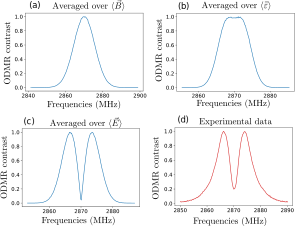
\includegraphics[width=\textwidth]{Figures/ESR_simus}
\caption{Simulations of inhomogeneous zero field ODMR when sampling various parameters. a) Simulation when sampling each components of the magnetic field over a Gaussian of deviation $\sigma=2\ \rm G$. b) Simulation when sampling each components of the strain tensor $\bar{\bar{\varepsilon}}$ over a Gaussian of deviation $\sigma=2\cdot 10^{-4}$. c) Simulation when sampling each components of the electric field over a Gaussian of deviation $\sigma=2\cdot 10^{5}\ \rm{V/cm}$. d) Experimental ODMR spectrum in zero external field taken on sample ADM-150-2}
\label{simus ESR}
\end{figure}

In the absence of external magnetic field, we have to take into account other elements which would otherwise be of second order in the spin Hamiltonian. These elements are: the random local magnetic fields caused by paramagnetic impurities, the local electric field caused by charged impurities, and the crystal strain \citep{doherty2012theory, udvarhelyi2018spin, mittiga2018imaging}. The hyperfine splitting due to nearby nuclei will be considered separately, although to a large extent it behaves like a local magnetic field.

Due to the large zero field splitting $D=2870 MHz$ between the $\ket{0}$ and $\ket{\pm 1}$ states, we will consider the $\ket{0}$ to always be an eigenstate of the spin Hamiltonian under zero external field (which is equivalent to say that we neglect the terms in $\ket{0}\bra{\pm 1}$ in the spin Hamiltonian). The problem is then reduced to the $\{ \ket{-1}, \ket{+1} \}$ subsystem.

The NV$^-$spin Hamiltonian in the $\{ \ket{-1}, \ket{+1} \}$ basis can be written as \citep{udvarhelyi2018spin}:
\begin{equation}
\mathcal{H}=\begin{pmatrix}
D-\gamma_e B_\parallel + f_\parallel(\mathbf{E}) + g_\parallel(\bar{\bar{\varepsilon}}) & f_\perp(\mathbf{E}) + g_\perp(\bar{\bar{\varepsilon}})\\
f^*_\perp(\mathbf{E}) + g^*_\perp(\bar{\bar{\varepsilon}})&D+\gamma_e B_\parallel + f_\parallel(\mathbf{E}) + g_\parallel(\bar{\bar{\varepsilon}})
\end{pmatrix},
\label{Hamiltonien pm1}
\end{equation}
where $B_\parallel$ is the component of the magnetic field along the NV axis, and $f_\parallel, f_\perp, g_\perp$, and $g_\parallel$ are functions of the electric field $\mathbf{E}$ and the strain tensor $\bar{\bar{\varepsilon}}$, whose expressions are:

\begin{align}
f_\parallel(\mathbf{E})&=d_\parallel E_z, \\
f_\perp(\mathbf{E})&=d_\perp ( E_x + i E_y), \\
g_\parallel(\bar{\bar{\varepsilon}})&= h_{41}(\varepsilon_{xx}+\varepsilon_{yy})+h_{43} \varepsilon_{zz}, \\
g_\perp(\bar{\bar{\varepsilon}}) &= \frac{1}{2} \left[ h_{16}(\varepsilon_{zx}+i \varepsilon_{zy}) + h_{15}\left(\frac{\varepsilon_{yy}-\varepsilon_{xx}}{2}+i\varepsilon_{xy}\right) \right],
\end{align}
where $d_\parallel=0.35 \ \rm{Hz\, cm/V}$ and $d_\perp=17\ \rm{Hz\, cm/V}$ have been measured experimentally \citep{van1990electric}, and $h_{43}=2300\ \rm{MHz}$, $h_{41}=-6420\ \rm{MHz}$, $h_{15}=5700\ \rm{MHz}$ and $h_{16}=19660\ \rm{MHz}$ were computed through DFT \citep{udvarhelyi2018spin} and show reasonable agreement with experiments \citep{barson2017nanomechanical}.

Importantly, as pointed in \citep{mittiga2018imaging} we notice that both the electric field and the strain have a \textit{shifting} component ($f_\parallel$ and $g_\parallel$) which shifts equally both eigenstates of the Hamiltonian, and a \textit{splitting} component ($f_\perp$ and $g_\perp$) which splits in energy the two eigenstates. 

The main difference between the electric field and the strain is in the numerical prefactors of these components: for the electric field, the splitting parameter $d_\perp$ is $\sim 50$ times higher than the shifting parameter $d_\parallel$, which will result on average to a strong energy split without much shifting. For the strain however, the splitting parameters $h_{15}$ and $h_{16}$ are only $\sim 3$ times higher than the shifting parameters $h_{43}$ and $h_{41}$. The shift in energy will therefore tend to blur the energy split when averaging over a large number of spins.

Fig. \ref{simus ESR} shows a simulation of how each parameters of the spin Hamiltonian - local magnetic field, local electric field and strain - affects the zero external field ODMR profile. To do these simulations, I sampled each parameters separately $10^6$ times and plotted the histogram of the two eigenvalues of the Hamiltonian written in eq. \ref{Hamiltonien pm1}. Fig. \ref{simus ESR}-d) shows an experimental zero field ODMR spectrum, typical of what we observe with dense NV ensembles. 

Experimentally, almost all our samples show the characteristic two bumps in zero external field ODMR. Given the simulation results, the only parameter that can give rise to this shape is the electric field. We will therefore consider that the NV Hamiltonian of our samples is dominated by the local electric field, and more specifically by the transverse electric field $E_\perp\equiv E_x + i E_y$ given the ratio between $d_\perp$ and $d_\parallel$.

We will then adopt the following simplified Hamiltonian for the zero external field regime:
\begin{equation}
\mathcal{H}=\begin{pmatrix}
D&0&d_\perp E_\perp^* \\
0&0&0 \\
d_\perp E_\perp &0&D
\end{pmatrix},
\end{equation}
whose eigenvectors are $\ket{0}$ and$\ket{\pm}$ of eigenvalues 0 and $D\pm d_\perp \abs{E_\perp}$, where $\ket{\pm}$ are defined as:
\begin{equation}
\ket{\pm}=\frac{\ket{+1}\pm e^{-i\phi_E}\ket{-1}}{\sqrt{2}},
\end{equation}
where $\tan(\phi_E)=E_y/E_x$.

\subsection{NV spin Hamiltonian under purely transverse magnetic field}

%\begin{figure}[h]
%\centering
%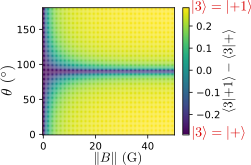
\includegraphics[width=0.7\textwidth]{Figures/map_etats_propres}
%\caption{Closeness of the Hamiltonian most excited state $\ket{3}$ with either $\ket{+1}$ or $\ket{+}$ as a function of the external magnetic field amplitude and angle $\theta$ with respect to the NV axis.}
%\label{map champ transverse}
%\end{figure}

We will consider here the case of purely transverse magnetic field with respect to the NV axis, i.e. $\mathbf{B}=B_x \hat{e}_x + B_y \hat e_y$, and more specifically the regime where $d_\perp E_\perp < \frac{(\gamma_e B_\perp)^2}{D} << D$. In practice, this generally means $20\ \rm G \lesssim B_\perp \lesssim 200\ \rm G$.

In this regime, the NV Hamiltonian eigenstates are similar to the case dominated by the transverse electric field and can be written $\approx \ket{0}, \ket{\pm}$\citep{qiu2021nuclear, qiu2022nanoscale}, of eigenvalues $\approx -\frac{(\gamma_e B_\perp)^2}{D},D$ and $D+\frac{(\gamma_e B_\perp)^2}{D}$,  where:
\begin{equation}
\ket{\pm}=\frac{\ket{+1}\pm e^{-2i\phi_B}\ket{-1}}{\sqrt{2}},
\end{equation}
and $\tan(\phi_B)=B_y/B_x$.

For the case where $d_\perp E_\perp \sim \frac{(\gamma_e B_\perp)^2}{D}$ and $\phi_E \neq 2\phi_B$, the eigenstates of the Hamiltonian are still $\ket{0},\ket{\pm}$ with a relative angle $\phi$ in between $\phi_E$ and $2\phi_B$.

In conclusion, whenever the spin Hamiltonian is dominated by a transverse field, either electric or magnetic, we can consider that the eigenstates of the spin Hamiltonian or $\ket{0}, \ket{-}$ and $\ket{+}$, whereas when the spin Hamiltonian is dominated by the longitudinal magnetic field, the spin eigenstates are $\ket{0}, \ket{-1}$ and $\ket{+1}$.

\subsection{Hyperfine coupling and inhomogeneous broadening}
Jambonneau mais pas que. Foutre des ESR si possible. Je vais en chier en vrai.

\section{Modification of NV-NV CR in the transverse field dominated regime}
In this part, we will study the cross-relaxation between NV centers whose spin Hamiltonian is dominated by a transverse field, either magnetic or electric. This is an important regime because it corresponds to the low magnetic field region where the electric field dominates, which is the region for which we want to implement our magnetometry protocol. We will also study here the double flip CR processes which we had neglected in the last chapter.

\subsection{NV-NV CR under low magnetic field}
\begin{figure}[h]
\centering
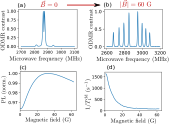
\includegraphics[width=0.9\textwidth]{Figures/scan_1x1x1x1}
\caption{tata. Changer les T1 avec T1ph=5ms}
\label{scan 1x1x1x1}
\end{figure}
We will start by showing that NV-NV CR behaves differently in the low magnetic field regime compared to the longitudinal field dominated regime which we studied in the last chapter.

The main issue with studying NV-NV CR in low to zero magnetic field is that there are many competing effects happening simultaneously, with few buttons to adjust to isolate each effects.

Fig. \ref{scan 1x1x1x1}-c) and d) for example shows the evolution of the NV PL and stretched lifetime $T_1^{\rm dd}$, defined in the last chapter [REF], as the magnetic field is scanned from 0 to 60 G. The ODMR at the initial and final magnetic fields are shown in Fig. \ref{scan 1x1x1x1}-a) and b).

While it is clear that the spin lifetime, as well as the PL, increases when the magnetic field, there is no clear indication that this is because of the specificity of the low field region. Indeed, the most likely explanation in this case is that the four classes of NV centers get split apart as the magnetic field increases, which reduces the density of resonant fluctuators for each NV centers.

\begin{figure}[h]
\centering
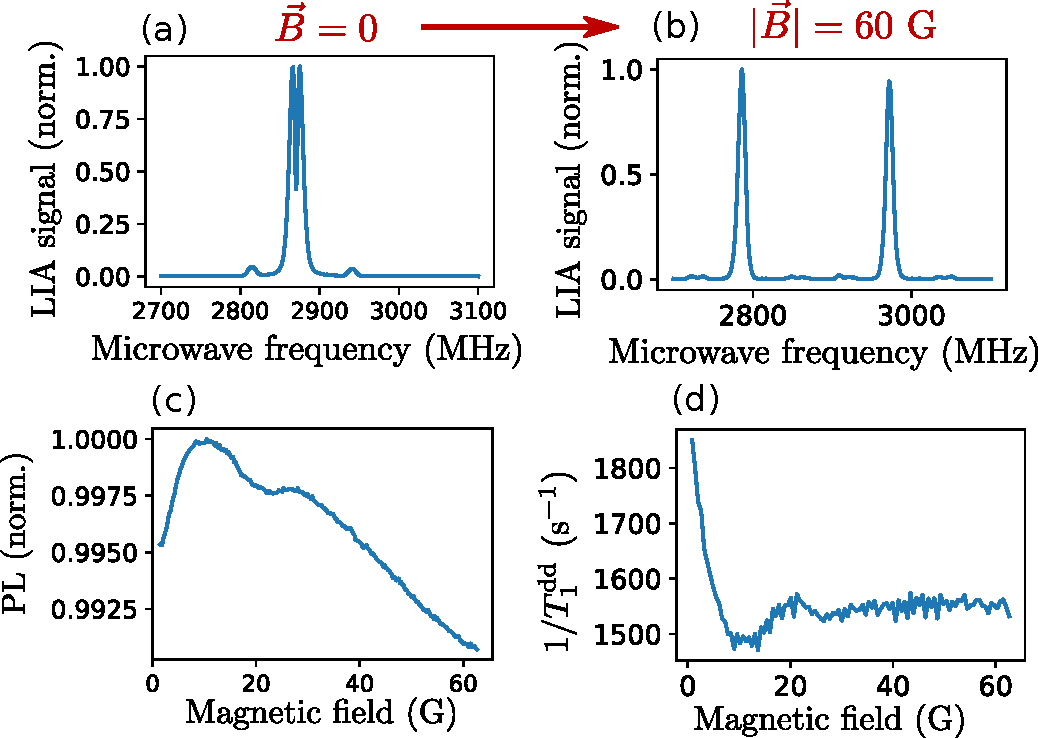
\includegraphics[width=0.9\textwidth]{Figures/scan_100}
\caption{Same measurements as Fig. \ref{scan 1x1x1x1}, still on sample ADM-150-1, but with $\mathbf{B}$ along the [100] axis. Changer les T1 avec T1ph=5ms}
\label{scan 100}
\end{figure}

Fig. \ref{scan 100} presents a way to circumvent this issue: by applying the magnetic field along the [100] crystalline axis, we can make sure that the four classes of NV centers always stay resonant regardless of the magnetic field amplitude.

We can notice that there still is a decrease of both the PL and $T_1^{\rm dd}$ in low field, although considerably smaller than the previous case: in Fig. \ref{scan 1x1x1x1}, $T_1^{\rm dd}$ was reduced by a factor of [REF] in zero field, whereas in Fig. \ref{scan 100}, it was only reduced by a factor of [REF]. The main reason for the PL and $T_1$ drop was indeed the co-resonance between the four classes.

Nevertheless, the fact that there is a drop in zero field when $\mathbf{B} \parallel [100]$ cannot be explained by using only the inter-class resonances. There are some additional depolarization mechanisms which are proper to the zero field region. We should also note that, while the zero-field PL contrast is bigger in Fig. \ref{scan 1x1x1x1}-c) than in Fig. \ref{scan 100}-c), the slope, which is the limiting factor for sensing ability, is actually very similar in both cases with a value $\sim [REF]\ \rm G^{-1}$.

\subsection{Potential causes for low field depolarization}

Tutut, tu fais le hyperfin avant de continuer.
\subsubsection{Change in eigenstates}

\subsubsection{Double flips}

\subsubsection{Change in $T_2^*$}

\subsection{NV-NV CR under purely transverse magnetic field}

Sa mère, faut que je replotte tous les T1 avec t1ph=5 ms.

\subsection{Other potential causes}
Alignment : 100 et perp (utiliser la carte)
Pola laser

\section{Low field magnetometry}

Ne pas oublier (ou alors en perspective, c'est bien aussi) : les deux adamas du 20210927 avec le petit et le gros 

\section{Conclusion and perspectives}
- Improvement to the sensitivity : Scale up, material optimization (15N !)

- Understand the impact of the various factors on the flip-flop CR and DQ CR: T2*, strain, local electric noise ...

- Application for uneven surfaces, polycrystalline heteroepithaxy, low/no microwave environment (dimaond anvil cells, bio sensing)

\printbibliography
\end{document}